% !TeX spellcheck = en_US
% !TeX encoding = UTF-8
% !TeX root = ../report.tex

\chapter{Modeling}
\label{chp:modeling}

In this chapter, the mathematical models of the solar car are derived. They are necessary for understanding the relation between the various components. Second, the data used to represent the race track is presented. This includes time- and location-dependent quantities like inclination, ambient temperature, and solar irradiance. Lastly, the relevant rules are listed.


\section{Vehicle}

\subsection{Longitudinal Vehicle Dynamics}
\label{sec:modelLVD}
According to Newtown's second law, the longitudinal vehicle dynamics (LVD) are described by the following differential equation~\cite{vps:2007book, sutteben:2017mt}.
\begin{equation}
	m_\mathrm{tot} \cdot \frac{\mathrm{d}}{\;\mathrm{d}t} v(t) = F_\mathrm{trac}(t) - \left(F_\mathrm{aero}(t) + F_\mathrm{roll}(t) + F_\mathrm{grav}(t) + F_\mathrm{bear}\right),
\end{equation}
where $m_\mathrm{tot}$ is the total mass, $v$ is the car velocity, $F_\mathrm{trac}$ is the traction force generated by the motor and is modeled in~\cref{sec:modelMotor},
$F_\mathrm{aero}$ is the aerodynamic friction force, $F_\mathrm{roll}$ is the rolling friction force, $F_\mathrm{grav}$ is the gravitational force, and $F_\mathrm{bear}$ is the bearing friction force. All forces are schematically shown in~\cref{fig:lvd}.
\begin{figure}[htbp]
	\centering
	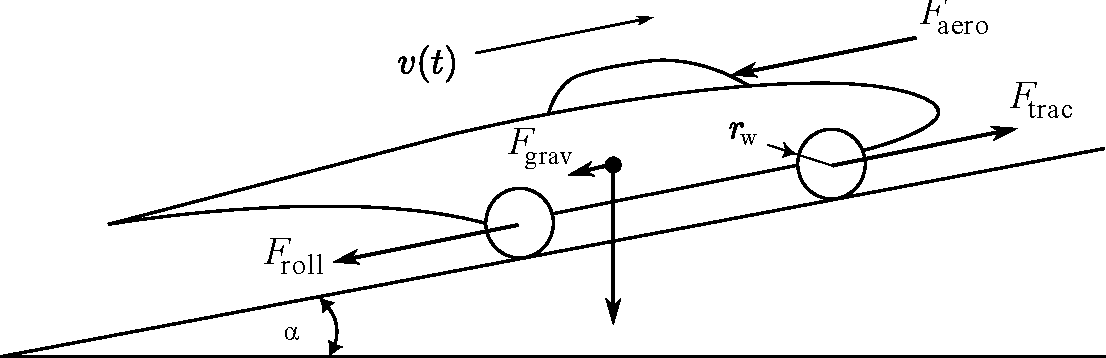
\includegraphics[width=0.75\textwidth, height=0.25\textwidth]{img/lvd/lvd.pdf}
	\caption{Schematic of the LVD.}
	\label{fig:lvd}
\end{figure}

Alternatively, the vehicle can be thought of as an energy reservoir: the motor produces mechanical energy that is stored in it, while the resistances consume energy that is irreversibly lost in heat.

The resistance forces are modeled as follows:
\begin{align}
	F_\mathrm{aero} &= \frac{1}{2} \cdot \rho_\mathrm{air} \cdot A_\mathrm{front} \cdot c_\mathrm{aero} \cdot v_\mathrm{eff,front}(t)^2 \\
	F_\mathrm{roll} &= c_\mathrm{roll} \cdot m_\mathrm{tot} \cdot g \cdot \cos(\alpha(t)) \quad , \quad v > 0 \\
	F_\mathrm{grav} &= m_\mathrm{tot} \cdot g \cdot \sin(\alpha(t)) \\
	F_\mathrm{bear} &= N_\mathrm{front} \cdot \frac{T_\mathrm{front}}{r_\mathrm{w}} + N_\mathrm{rear} \cdot \frac{T_\mathrm{rear}}{r_\mathrm{w}}
\end{align}


where $\rho_\mathrm{air}$ is the air density, $A_\mathrm{front}$ is the frontal area, $c_\mathrm{aero}$ is the aerodynamic drag coefficient, $v_\mathrm{eff,front}$ is the frontal effective velocity which accounts for the relative car velocity with respect to the frontal wind and it is derived in~\cref{sec:windSpeed}, $c_\mathrm{roll}$ is the rolling friction coefficient, $g$ is the gravitational constant, $\alpha$ is the inclination of the road, $N_\mathrm{front}$ and $N_\mathrm{rear}$ are the numbers of front and back bearings, $T_\mathrm{front}$ and $T_\mathrm{rear}$ are the front and back friction torque of the bearings, and $r_\mathrm{w}$ is the wheel radius.

Here, both the aerodynamic drag coefficient $c_\mathrm{aero}$ and the rolling friction coefficient $c_\mathrm{roll}$ are assumed constant. In reality however, the former is typically a function of velocity, while the latter depends on velocity, ambient temperature, and pressure.

The total mass of the vehicle is found as the sum of the mass contributions:
\begin{equation}
	m_\mathrm{tot} = m_\mathrm{car} + m_\mathrm{driver} + m_\mathrm{rot}
\end{equation}
where $m_\mathrm{car}$ is the mass of the solar car, $m_\mathrm{driver}$ is the driver mass, $m_\mathrm{rot}$ is the equivalent rotational mass of the drivetrain. The influence of rotating parts on the inertia of the vehicle is modeled in~\cite{optimalEnergyManagement:2000book, vps:2007book} as follows:
\begin{equation}
	m_\mathrm{rot} = \frac{\Theta_\mathrm{rot}}{r_\mathrm{w}^2}
\end{equation}
where $\Theta_\mathrm{rot}$ is the moment of inertia (MOI) of all rotating parts. The rotational mass adds around $\unit[14]{kg}$ to the total mass.

The parameters for the considered vehicle and their numerical values are listed in~\cref{tab:modelingParametersLVD}.
\begin{table}[htbp]
	\centering
	\caption{Modeling parameters for the LVD.}
	\label{tab:modelingParametersLVD}
	
	\begin{tabular}{l l r l}
		\toprule
		Parameter                       		& Symbol                & Value 	& Unit\\ 
		\midrule
		Air density 							& $\rho_\mathrm{air}$   & 1.17     	& \unitfrac{kg}{m$^3$} \\
		Frontal area 							& $A_\mathrm{front}$    & 0.8   	& \unit{m$^2$} \\
		Aerodynamic drag coefficient 			& $c_\mathrm{aero}$     & 0.07     	& -- \\
		Rolling friction coefficient 			& $c_\mathrm{roll}$     & 0.003    	& -- \\
		Total mass 								& $m_\mathrm{tot}$   	& 220    	& \unit{kg} \\
		Gravitational acceleration 				& $g$         			& 9.81     	& \unitfrac{m}{s$^2$} \\
		Wheel radius 							& $r_\mathrm{w}$ 		& 27.85    	& \unit{cm} \\
		Number of front bearings 				& $N_\mathrm{front}$ 	& 4 		& -- \\
		Friction torque in one front bearing 	& $T_\mathrm{front}$ 	& 0.0550 	& \unit{N$\,$m} \\
		Number of back bearings 				& $N_\mathrm{rear}$ 	& 1 		& -- \\
		Friction torque in the back bearing 	& $T_\mathrm{rear}$ 	& 0.15 		& \unit{N$\,$m} \\
		Car mass 								& $m_\mathrm{car}$      & 150   	& \unit{kg} \\
		Driver mass 							& $m_\mathrm{driver}$   & 80    	& \unit{kg} \\
		MOI of rotating parts 					& $\Theta_\mathrm{rot}$ & 1.1343	& \unit{kg$\,$m$^2$} \\
		\bottomrule
	\end{tabular}
\end{table}


\subsection{Electric Motor}
\label{sec:modelMotor}
The traction force needed to accelerate the car can be linked to the electric power consumption via a model of the drivetrain.~\Cref{fig:drivetrain} illustrates the relevant variables and parameters used for this purpose.
\begin{figure}[htbp]
	\centering
	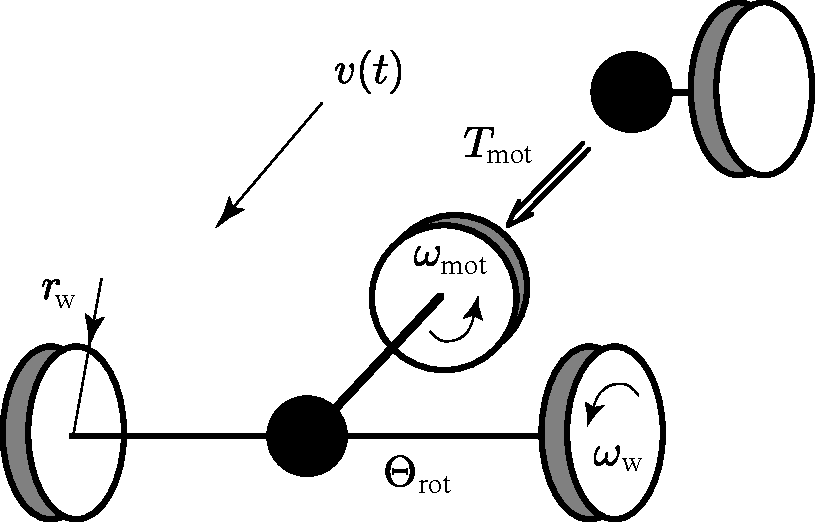
\includegraphics[width=0.5\textwidth, height=0.3\textwidth]{img/drivetrain/drivetrain3wheels.pdf}
	\caption{Schematic of the drivetrain without gear box and three wheels~\cite{SysMod:2022misc}.}
	\label{fig:drivetrain}
\end{figure}

Assuming perfect rigid bodies and lossless transmission, the drivetrain relations are modeled as follows~\cite{vps:2007book}:
\begin{align}
	P_\mathrm{mot,mec} &= T_\mathrm{mot}(t) \cdot \omega_\mathrm{mot}(t) = F_\mathrm{trac}(t) \cdot v(t) \label{eq:motorMechPower}\\
	\omega_\mathrm{mot} &= \gamma_\mathrm{gb} \cdot \omega_\mathrm{w}(t) = \gamma_\mathrm{gb} \cdot \frac{v(t)}{r_\mathrm{w}} \label{eq:motorAngularVelocity}
\end{align}
where $P_\mathrm{mot,mec}$ is the mechanical power generated by the motor, $T_\mathrm{mot}$ is the motor torque, $\omega_\mathrm{mot}$ is the rotational velocity of the motor, $\omega_\mathrm{w}$ is the rotational velocity of the wheel, and $\gamma$ is the transmission ratio.

Inserting~\cref{eq:motorAngularVelocity} in ~\cref{eq:motorMechPower} and solving for the motor torque yields:
\begin{equation}
	T_\mathrm{mot} = F_\mathrm{trac}(t) \cdot \frac{r_\mathrm{w}}{\gamma_\mathrm{gb}}
\end{equation}
The motor torque is bounded by component limitations:
\begin{equation}
	T_\mathrm{mot,min} \leq T_\mathrm{mot} \leq T_\mathrm{mot,max}.
\end{equation}

To connect the mechanical output power $P_\mathrm{mot,mec}$ with the electrical input power to the motor $P_\mathrm{mot,el}$, the Willans model can be exploited~\cite{vps:2007book}, where a linear relation is used:
\begin{equation}
	P_\mathrm{mot,mec} =
\begin{cases}
	e_\mathrm{mot} \cdot P_\mathrm{mot,el}(t) - P_0 \qquad & \text{if} \quad P_\mathrm{mot,el} \geq 0 \quad , \quad \text{Traction,} \\
	\frac{P_\mathrm{mot,el}(t)}{e_\mathrm{mot}} - P_0 \qquad & \text{if} \quad P_\mathrm{mot,el} < 0 \quad , \quad \text{Regeneration.}
\end{cases}
\label{eq:motorWillansMechPower}
\end{equation}
where $e_\mathrm{mot}$ is the motor efficiency, and $P_0$ is the idle power loss.

Solving~\cref{eq:motorWillansMechPower} for the electric power yields:
\begin{equation}	
	P_\mathrm{mot,el} =
	\begin{cases}
		\frac{P_\mathrm{mot,mec}(t) + P_0}{e_\mathrm{mot}} \qquad & \text{if} \quad P_\mathrm{mot,mec} \geq -P_0 \quad , \quad \text{Traction,} \\
		e_\mathrm{mot} \cdot \left(P_\mathrm{mot,mec}(t) + P_0 \right) \qquad & \text{if} \quad P_\mathrm{mot,mec} < -P_0 \quad , \quad \text{Regeneration.}
	\end{cases}
\end{equation}
The electric power is also limited by
\begin{equation}
	P_\mathrm{mot,el,min} \leq P_\mathrm{mot,el} \leq P_\mathrm{mot,el,max}
\end{equation}

The parameters and their numerical values are listed in~\cref{tab:modelingParametersMotor}.
\begin{table}[htbp]
	\centering
	\caption{Modeling parameters for the electric motor.}
	\label{tab:modelingParametersMotor}
	
	\begin{tabular}{l l r l}
		\toprule
		Parameter 								& Symbol 					& Value & Unit\\ 
		\midrule
		Transmission ratio through the gear box & $\gamma_\mathrm{gb}$      & 1     & -- \\
		Motor efficiency 						& $e_\mathrm{mot}$      	& 0.97  & -- \\
		Idle losses 							& $P_0$      				& 30    & \unit{W} \\
		Maximal electric power 					& $P_\mathrm{mot,el,max}$	& 5000  & \unit{W} \\
		Minimal electric power 					& $P_\mathrm{mot,el,min}$   & -5000 & \unit{W} \\
		Maximal torque 							& $T_\mathrm{mot,max}$      & 45    & \unit{N$\,$m} \\
		Minimal torque 							& $T_\mathrm{mot,min}$      & -45   & \unit{N$\,$m} \\
		\bottomrule
	\end{tabular}
\end{table}


\subsection{Photovoltaic Module}
\label{sec:modelPV}
The solar radiation is converted into electrical power using photovoltaic panels mounted on top of the car bodywork. The relevant variables and parameters are schematically shown in~\cref{fig:PVmodel}.
\begin{figure}[htbp]
	\centering
	\tikzstyle{PVarray} = [thick,black]
\tikzstyle{arrow} = [thick, ->, >=stealth]
\tikzstyle{sun} = [thick, ->, >=stealth,red]
\tikzstyle{wind} = [thick, ->, >=stealth,blue]

\begin{tikzpicture}[
	thick,
	>=stealth',
	dot/.style = {
		draw,
		fill = white,
		circle,
		inner sep = 0pt,
		minimum size = 4pt
	}
	]
	% Origin
	\coordinate (Origin) at (0,0);
	% Data points
	\coordinate (b1) at (1,0);
	\coordinate (b2) at (2,0);
	\coordinate (b3) at (3,0);
	\coordinate (b4) at (4,0);
	\coordinate (b5) at (5,0);
	\coordinate (v1) at ({-2/3},0.5);
	\coordinate (v2) at ({-4/3},1);
	\coordinate (v3) at (-2,1.5);
	
	% PV array
	\draw[PVarray] (Origin) -- (b4);
	\draw[PVarray,dashed] (b4) -- (b5);
	\draw[PVarray] let \p1=(v3) in (3,\y1) -- (v3) node[above,black] {$A_\mathrm{PV}$};
	\draw[PVarray,dashed] (3,1.5) -- (4,1.5);
	\draw[PVarray] let \p1=(v1) in ({17/6},\y1) -- (v1);
	\draw[PVarray,dashed] let \p1=(v1) in ({17/6},\y1) -- ({17/6+1},\y1);
	\draw[PVarray] let \p1=(v2) in ({13/6},\y1) -- (v2);
	\draw[PVarray,dashed] let \p1=(v2) in ({13/6},\y1) -- ({13/6+1},\y1);
	%vertical
	\draw[PVarray] (Origin) -- (v3);
	\draw[PVarray] let \p1=(v3) in (-1,\y1) -- (b1);
	\draw[PVarray] let \p1=(v3) in (0,\y1) -- (b2);
	\draw[PVarray] let \p1=(v3) in (1,\y1) -- (b3);
	\draw[PVarray,dashed] let \p1=(v3) in (2,\y1) -- (b4);

	
	% Name
	\node[black] at (5,0.8) {$\vartheta_\mathrm{PV}$, $\eta_\mathrm{PV}$};
	\node[black] at (-1.5,0) {$\vartheta_\mathrm{amb}$};
	
	% Wind
	\draw[wind] (4,1.8) node[above,blue] {$v_\mathrm{eff}$} -- (0.5,0.8);
	
	% Sun ray
	\draw[sun] (-2,3) -- (0,1.3) node[midway,right,red,xshift=0.5cm] {$G$};
	
	% Arrows below
	\draw[thick,black] (2,0) -- (2,-1)  node[midway,left, black] {$\eta_\mathrm{loss}$};
	\draw[arrow] (2,-1) -- (3,-1) node[above, black] {$P_\mathrm{PV}$};
	
\end{tikzpicture}
	\caption{Schematic representation of the PV module on the top of the car.}
	\label{fig:PVmodel}
\end{figure}

The model equation is the following~\cite{PVmodelling:2022misc}:
\begin{equation}
	P_\mathrm{PV} = A_\mathrm{PV} \cdot G(t) \cdot \eta_\mathrm{PV} \cdot \eta_\mathrm{CF}(t) \cdot \eta_\mathrm{loss}
\end{equation}
where $P_\mathrm{PV}$ is the power generated by the photovoltaic panels, $A_\mathrm{PV}$ is the area of the panels, $G$ is the total global irradiance, $\eta_\mathrm{PV}$ is the efficiency of the panels, $\eta_\mathrm{CF}$ is the temperature correcting factor, and $\eta_\mathrm{loss}$ is the conversion loss coefficient. The latter is equal to the multiplication of all efficiency losses in the PV conversion system~\cite{PVlosses:2017article}:
\begin{equation}
	\eta_\mathrm{loss} = \eta_\mathrm{wire} \cdot \eta_\mathrm{MPPT} \cdot \eta_\mathrm{mismatch}
\end{equation}
where $\eta_\mathrm{wire}$ accounts for losses inside the wires, $\eta_\mathrm{MPPT}$ accounts for losses caused by imprecision of the MPPT device, and $\eta_\mathrm{mismatch}$ accounts for losses caused by an off-set operation from the maximum power point.

The influence of the ambient temperature is modeled in $\eta_\mathrm{CF}$ as follows~\cite{PVmodelling:2022misc}:
\begin{equation}
	\eta_\mathrm{CF} = 1 - \lambda_\mathrm{PV} \cdot \left( \vartheta_\mathrm{PV}(t) - \vartheta_\mathrm{STC} \right)
\end{equation}
where $\lambda_\mathrm{PV}$ is the power loss coefficient, $\vartheta_\mathrm{STC}$ is the standard condition temperature, and $\vartheta_\mathrm{PV}$ is the temperature of the panels. As explained in~\cite{PVmodelling:2022misc}, many models are available to describe the temperature of the panels. Here, the Sandia model for module temperature is chosen, since it includes the dependency on the wind speed:
\begin{equation}
	\vartheta_\mathrm{PV} = G(t) \cdot \exp\left(\nu + \kappa \cdot v_\mathrm{eff}(t)\right) + \vartheta_\mathrm{amb}(t) + \frac{G(t)}{G_\mathrm{0}} \cdot \Delta \vartheta \label{eq:modelingPVtempPV}
\end{equation}
where $\nu, \kappa, \Delta \vartheta$ are coefficients read from~\cref{tab:modelingParametersPVSandia}, $v_\mathrm{eff}$ is the effective air velocity cooling the panels which accounts for both car velocity and wind contribution and is derived in~\cref{sec:windSpeed}, $\vartheta_\mathrm{amb}$ is the ambient temperature, and $G_\mathrm{0}$ is the reference global irradiance. 
\begin{table}[htbp]
	\centering
	\caption{Parameters for the module temperature equation using Sandia model taken from~\cite{PVmodelling:2022misc, PVlosses:2017article}.}
	\label{tab:modelingParametersPVSandia}
	
	\begin{tabular}{l l c c c}
		\toprule
		Module Type 				& Mounting 			& $\nu$ / -- 	& $\kappa$ / $\unitfrac{s}{m}$ & $\Delta \vartheta$ / $\unit{\celsius}$ \\ 
		\midrule
		Glass-cell-glass 			& Open rack 		& -3.47 	& -0.0594 				& 3 \\
		Glass-cell-glass 			& Close roof mount 	& -2.98 	& -0.0471 				& 1 \\
		Glass-cell-polymer sheet 	& Open rack 		& -3.56 	& -0.0750 				& 3 \\
		Glass-cell-polymer sheet 	& Insulated back 	& -2.81 	& -0.0455 				& 0 \\
		Polymer-thin film-steel 	& Open rack 		& -3.58 	& -0.1130 				& 3 \\
		\bottomrule
	\end{tabular}
\end{table}

The first row of~\cref{tab:modelingParametersPVSandia} is used, since it is assumed that internal cooling system resembles an open rack configuration with free convection cooling.

The remaining parameters and their numerical values are listed in~\cref{tab:modelingParametersPV}.
\begin{table}[htbp]
	\centering
	\caption{Modeling parameters for the photovoltaic modules.}
	\label{tab:modelingParametersPV}
	
	\begin{tabular}{l l r l}
		\toprule
		Parameter 						& Symbol 					& Value 	& Unit\\ 
		\midrule
		Solar panels area 				& $A_\mathrm{PV}$       	& 4     	& \unit{m$^2$} \\
		Solar panels efficiency 		& $\eta_\mathrm{PV}$      	& 0.244   	& -- \\
		Wiring efficiency 				& $\eta_\mathrm{wire}$      & 0.98    	& -- \\
		MPPT efficiency 				& $\eta_\mathrm{MPPT}$      & 0.99    	& -- \\
		Mismatch efficiency 			& $\eta_\mathrm{mismatch}$  & 0.98    	& -- \\
		Standard-condition temperature 	& $\vartheta_\mathrm{STC}$      	& 25     	& \unit{\celsius} \\
		Reference global irradiance 	& $G_\mathrm{0}$      		& 1000    	& \unitfrac{W}{m$^2$} \\
		Power loss coefficient 			& $\lambda_\mathrm{PV}$      & 0.0029	& \unitfrac{1}{\celsius} \\
		\bottomrule
	\end{tabular}
\end{table}


\subsection{Battery Pack}
\label{sec:modelBattery}
The energy storage of the car is represented by a pack of \ce{Li}-ion batteries with a maximum energy capacity of $\unit[5000]{Wh}$, which is imposed by the rules of the competition.

The battery pack is modeled by considering an equivalent circuit with an internal resistance in series with an ideal open-circuit voltage as shown in~\cref{fig:batteryModel}~\cite{vps:2007book, sutteben:2017mt, fawidmer:2016mt}.
\begin{figure}[htbp]
	\centering
	\begin{circuitikz}
	
	\draw (0,0) to [american voltage source, l_=$U_\mathrm{bat,oc}$] (0,3);
	\draw (0,3) to [resistor, l^=$R_\mathrm{bat}$, -o] (4,3);
	\draw (0,0) to [short,i<=$I_\mathrm{bat}$,-o] (4,0);
	\draw (4,3) to[open, v^>=\mbox{ }$U_\mathrm{bat}$] (4,0);
	
\end{circuitikz}
	\caption{Equivalent circuit of the battery pack~\cite{IDSCreportClass:2021manual}.}
	\label{fig:batteryModel}
\end{figure}

Using Kirchhoff's voltage law, the following relation is found.
\begin{equation}
	U_\mathrm{bat} = U_\mathrm{bat,oc} - R_\mathrm{bat} \cdot I_\mathrm{bat}(t) \label{eq:batteryVoltage}
\end{equation}
where $U_\mathrm{bat}$ is the battery pack voltage, $U_\mathrm{bat,oc}$ is the open-circuit voltage, $R_\mathrm{bat}$ is the internal resistance, and $I_\mathrm{bat}$ is the battery pack current.

The power from and to the battery pack ($P_\mathrm{bat}$) is described with the following equation that directly allows the integration of physical constraints.
\begin{align}
	P_\mathrm{bat} &= U_\mathrm{bat}(t) \cdot I_\mathrm{bat}(t) \quad
	\begin{cases}
		> 0 \qquad & , \quad \text{Discharge,} \\
		< 0 \qquad & , \quad \text{Charge.} \\
	\end{cases} \label{eq:batteryPower} \\
	P_\mathrm{bat,min} \leq P_\mathrm{bat} &\leq P_\mathrm{bat,max}
\end{align}

Inserting~\cref{eq:batteryVoltage} in~\cref{eq:batteryPower} and solving the quadratic equation for the current leads to
\begin{equation}
	I_\mathrm{bat} = \frac{U_\mathrm{bat,oc} \pm \sqrt{U_\mathrm{bat,oc}^2 - 4 \cdot R_\mathrm{bat} \cdot P_\mathrm{bat}(t)}}{2 \cdot R_\mathrm{bat}} \\
\end{equation}
The only physical result is the one with the minus sign, since $I_\mathrm{bat} = 0$ results for $P_\mathrm{bat} = 0$. Component limitations are considered here as well:
\begin{equation}
	I_\mathrm{bat,min} \leq I_\mathrm{bat} \leq I_\mathrm{bat,max}.
\end{equation}

Furthermore, in order to avoid nonphysical complex values, the term under the square root has to be non-negative. This requirement yields an additional condition for the battery power:
\begin{equation}
	P_\mathrm{bat} \leq \frac{U_\mathrm{bat,oc}^2}{4 \cdot R_\mathrm{bat}}. \label{eq:modelBatLimitSQRT}
\end{equation}

The charge level of the battery is represented by its state of charge (SoC), which can naturally only take values from 0 to 100\%. The SoC evolves according to the following differential equation.
\begin{equation}
	x_\mathrm{SoC} = \frac{1}{Q_\mathrm{bat,max}} \cdot \int \dot{Q}_\mathrm{bat}(t) \;\mathrm{d}t \quad \in [0,1]
\end{equation}
where $Q_\mathrm{bat,max}$ is the maximal capacity of the battery found with
\begin{equation}
	Q_\mathrm{bat,max} = \frac{E_\mathrm{bat,max}}{U_\mathrm{bat,oc}},
\end{equation}
where $E_\mathrm{bat,max}$ is the maximal energy capacity. Additionally, $\dot{Q}_\mathrm{bat}$ is the charge flow modeled as follows:
\begin{equation}
	\dot{Q}_\mathrm{bat} = - \eta_\mathrm{c} \cdot I_\mathrm{bat}(t),
\end{equation}
where $\eta_\mathrm{coul}$ is the coulombic efficiency that denotes the fraction of the current that is not transformed into charge due to irreversible, parasitic reactions.

Moreover, the constraints of minimal and maximal allowed SoC serve as safety bounds, since the batteries could become dangerously unstable outside of them:
\begin{equation}
	x_\mathrm{SoC,min} \leq x_\mathrm{SoC} \leq x_\mathrm{SoC,max}.
\end{equation}

All the parameters shown in~\cref{tab:modelingParametersBattery} are expressed for the whole battery pack.
\begin{table}[htbp]
	\centering
	\caption{Modeling parameters for the battery pack.}
	\label{tab:modelingParametersBattery}
	
	\begin{tabular}{l l r l}
		\toprule
		Parameter 				& Symbol 				& Value 	& Unit\\ 
		\midrule
		Open-circuit voltage 	& $U_\mathrm{bat,oc}$   & 126     	& \unit{V} \\
		Internal resistance 	& $R_\mathrm{bat}$      & 75   		& \unit{m$\Omega$} \\
		Maximal energy capacity	& $E_\mathrm{bat,max}$  & 5000    	& \unit{Wh} \\
		Maximal current 		& $I_\mathrm{bat,max}$  & 78.4    	& \unit{A} \\
		Minimal current 		& $I_\mathrm{bat,min}$  & -39.2    	& \unit{A} \\
		Maximal power 			& $P_\mathrm{bat,max}$  & 9878.4    & \unit{W} \\
		Minimal power 			& $P_\mathrm{bat,min}$  & -4939.4	& \unit{W} \\
		Maximal safe SoC		& $x_\mathrm{SoC,max}$  & 1    		& -- \\
		Minimal safe SoC 		& $x_\mathrm{SoC,min}$  & 0.1  		& -- \\
		Coulombic efficiency	& $\eta_\mathrm{coul}$		& 1			& -- \\
		\bottomrule
	\end{tabular}
\end{table}


\subsection{Power Balance}
\label{sec:modelPowerBalance}
As the battery is the only energy buffer in the vehicle powertrain, the power consumed by the motor minus the power generated by the PV panels has to be matched with the battery power:
\begin{equation}
	P_\mathrm{bat} = P_\mathrm{mot,el} - P_\mathrm{PV} \label{eq:powerBalance}
\end{equation}

\newpage
\section{Route on Stuart Highway}
\label{sec:modelingRouteData}
To ensure the validity of the results obtained in simulations, it is crucial to utilize data accurately represents the real driving route. This section presents the analysis and graphical representations of route information obtained from the \textit{Brouter} webpage~\cite{brouter:2022webpage}, including the coordinates of the road, the altitude, and the speed limit.


\subsection{Longitude, Latitude, and Distance}
The geographic trajectory of the route are fundamental to calculate accurate curved distances. Additionally, due to the high level of resolution of the \textit{Brouter} data, they will serve as the reference for space-dependent weather data of~\cref{sec:modelingWeatherData}.


\subsection{Altitude}
The altitude profile shown in~\cref{fig:altitude} is critical for estimating the inclination of the road as explained in~\cref{sec:modelingInclination} and calculating potential energy as in~\cref{sec:strategySpaceDomain}. To obtain more realistic results, the discrete noisy data is smoothed using the Matlab function \texttt{smooth}.
\begin{figure}[htbp]
	\centering
	% This file was created by matlab2tikz.
%
%The latest updates can be retrieved from
%  http://www.mathworks.com/matlabcentral/fileexchange/22022-matlab2tikz-matlab2tikz
%where you can also make suggestions and rate matlab2tikz.
%
%This file has been created via figure2tikz on 22-Dec-2022 20:44:56.
%
\begin{tikzpicture}

\begin{axis}[%
width=\textwidth,
height=0.3\textwidth,
xmin=0,
xmax=3000,
%xlabel style={font=\color{white!15!black}},
xtick={0,500,1000,1500,2000,2500,3000},
xticklabels={0,500,1000,1500,2000,2500,3000},
xlabel={Distance / km},
ymin=0,
ymax=800,
ylabel style={font=\color{white!15!black}},
ylabel={Altitude / m},
axis background/.style={fill=white},
grid=both,
]
\addplot [color=black, thick, forget plot]
  table[]{img/altitude/altitude-1.tsv};
\end{axis}
\end{tikzpicture}%
	\caption{Smoothed data of the altitude along the track.}
	\label{fig:altitude}
\end{figure}


\subsection{Inclination}
\label{sec:modelingInclination}
To calculate the slope of the road, we require longitude and latitude data to determine the distance between locations, as well as altitude information:
\begin{equation}
	\alpha_i = \arctan\left(\frac{h_{i+1} - h_i}{d_{i+1} - d_i} \right) \label{eq:inclination}
\end{equation}
where $h$ is the altitude, $d$ is the distance, and $i$ is the index.~\Cref{fig:inclinationTriangle} illustrates the schematic representation of the variables used in~\cref{eq:inclination}.
\begin{figure}[htbp]
	\centering
	\begin{tikzpicture}[thick,>=stealth']
	% Origin
	\coordinate (Origin) at (0,0);
	% Data points
	\coordinate (i-1) at (0.8,0.3);
	\coordinate (i) at (2.5,1);
	\coordinate (i+1) at (5,2);
	\coordinate (i+2) at (6.8,2.2);
	\coordinate (baseLinePoint) at (5,1);
	
	% Helping vertical lines
	\draw[gray,dashed] let \p1=(i) in (\x1,0) node[below, black] {$d_i$} -- (i);
	\draw[gray,dashed] let \p1=(i+1) in (\x1,0) node[below, black] {$d_{i+1}$} -- (i+1);
	% Helping horizontal lines
	\draw[gray,dashed] let \p1=(i) in (0,\y1) node[left, black] {$h_i$} -- (baseLinePoint);
	\draw[gray,dashed] let \p1=(i+1) in (0,\y1) node[left, black] {$h_{i+1}$} -- (i+1);
%	\draw[gray] (i) -- (baseLinePoint);
%	\draw[gray,dashed, name intersections={rightHelpLine}] let \p1=(i+1) in (0,\y1) node[left, black] {$h_{i+1}$} -- (i+1);
%	\draw (i) -- (i+1 |- rightHelpLine);

	% Angle
	\tkzMarkAngle[thin](baseLinePoint,i,i+1)
	\tkzLabelAngle[pos=1.3](baseLinePoint,i,i+1){$\alpha_i$}
	
	% Axis
	\draw[->] (Origin) -- coordinate (x axis mid) (8,0);
	\draw[->] (Origin) -- coordinate (y axis mid) (0,3);
	% Axis labels
	\node[below=0.55] at (x axis mid) {$d$ / $\unit{m}$};
	\node[rotate=90,yshift=40pt] at (y axis mid) {$h$ / $\unit{m}$};
	
	% Data lines
	\draw [lightgray,dashed] (i-1) -- (i);
	\draw [black] (i) -- (i+1);
	\draw [lightgray,dashed] (i+1) -- (i+2);
	% Data dots
	\fill [gray] (i-1) circle (0.07cm);
	\fill [black] (i) circle (0.07cm);
	\fill [black] (i+1) circle (0.07cm);
	\fill [gray] (i+2) circle (0.07cm);
\end{tikzpicture}
	\caption{Graphical representation of the inclination estimation.}
	\label{fig:inclinationTriangle}
\end{figure}

The estimated inclination data is visualized in~\cref{fig:inclination}.
\begin{figure}[htbp]
	\centering
	% This file was created by matlab2tikz.
%
%The latest updates can be retrieved from
%  http://www.mathworks.com/matlabcentral/fileexchange/22022-matlab2tikz-matlab2tikz
%where you can also make suggestions and rate matlab2tikz.
%
%This file has been created via figure2tikz on 22-Dec-2022 21:10:56.
%
\begin{tikzpicture}

\begin{axis}[%
width=\textwidth,
height=0.3\textwidth,
xmin=0,
xmax=3000,
%xlabel style={font=\color{white!15!black}},
xtick={0,500,1000,1500,2000,2500,3000},
xticklabels={0,500,1000,1500,2000,2500,3000},
xlabel={Distance / km},
ymin=-3,
ymax=3,
%ylabel style={font=\color{white!15!black}},
ytick={-3,-2,-1,0,1,2,3},
yticklabels={-3,-2,-1,0,1,2,3},
ylabel={Inclination / °},
axis background/.style={fill=white},
grid=both,
]
\addplot [color=black, forget plot]
  table[]{img/inclination/inclination-1.tsv};
\end{axis}
\end{tikzpicture}%
	\caption{Estimated road inclination along the track.}
	\label{fig:inclination}
\end{figure}
%This last plot indicates that the track is never particularly steep. Hence,~\cref{eq:lvdFrollApprpx} and~\cref{eq:lvdFgravApprpx} could be used, resulting in a smaller simulation running time and improvement of the computational effort.


\subsection{Speed Limit}
To comply with traffic regulations, it is necessary to adhere to the maximum allowed speed at all times.~\Cref{fig:speedLimit} shows the speed limit as a function of distance.
\begin{figure}[htbp]
	\centering
	\begin{externalize}{speedLimit}
		% This file was created by matlab2tikz.
%
%The latest updates can be retrieved from
%  http://www.mathworks.com/matlabcentral/fileexchange/22022-matlab2tikz-matlab2tikz
%where you can also make suggestions and rate matlab2tikz.
%
%This file has been created via figure2tikz on 22-Dec-2022 21:36:06.
%
\begin{tikzpicture}

\begin{axis}[%
width=\textwidth,
height=0.3\textwidth,
xmin=0,
xmax=3000,
%xlabel style={font=\color{white!15!black}},
xtick={0,500,1000,1500,2000,2500,3000},
xticklabels={0,500,1000,1500,2000,2500,3000},
xlabel={Distance / km},
ymin=40,
ymax=140,
ylabel style={font=\color{white!15!black}},
ylabel={Speed limit / $\unitfrac{km}{h}$},
axis background/.style={fill=white},
grid=both,
]
\addplot [color=black, thick, forget plot]
  table[]{img/speedLimit/speedLimit-1.tsv};
\end{axis}
\end{tikzpicture}%
	\end{externalize}
	\caption{Maximal allowed driving speed along the track.}
	\label{fig:speedLimit}
\end{figure}
This visualization clearly shows that the majority of the track corresponds to a highway with relatively high speed limits. The downward spikes in the speed limit correspond to crossings of residential areas.


\newpage
\section{Meteorological Conditions}
\label{sec:modelingWeatherData}
In this section, the three weather variables influencing the models are presented: the global irradiance, ambient temperature, and wind speed characterized by intensity and direction.

Furthermore, since the route of the competition passes through three time zones in Australia, the time reference used in this report is based on the starting location in Darwin.


\subsection{Solar Global Irradiance}
To make the analysis of~\cref{chp:strategy} possible, the global irradiance data is taken from~\cite{irradianceData:2022webpage} as a function of time only. However, the usage of this high resolution data comes with the drawback that it is referred to a single specific year and not to more accurate mean values.

\Cref{fig:irradianceRace2020} shows the global irradiance as a function of time for the five October days of 2020, when the competition takes place.
\begin{figure}[htbp]
	\centering
	% This file was created by matlab2tikz.
%
%The latest updates can be retrieved from
%  http://www.mathworks.com/matlabcentral/fileexchange/22022-matlab2tikz-matlab2tikz
%where you can also make suggestions and rate matlab2tikz.
%
%This file has been created via figure2tikz on 20-Dec-2022 09:12:11.
%
\begin{tikzpicture}

\begin{axis}[%
width=\textwidth,
height=0.3\textwidth,
xmin=0,
xmax=7080,
%xlabel style={font=\color{white!15!black}},
xtick={0,1400,2850,4280,5720},
xticklabels={Oct 20,Oct 21,Oct 22,Oct 23,Oct 24},
xlabel={Time / days},
ymin=0,
ymax=1200,
%ylabel style={font=\color{white!15!black}},
ytick={0,300,600,900,1200},
yticklabels={0,300,600,900,1200},
ylabel={Global irradiance / $\unitfrac{W}{m^2}$},
axis background/.style={fill=white},
grid=both
]
\addplot [color=black, forget plot]
  table[]{img/irradianceRace2020/irradianceRace2020-1.tsv};
\end{axis}
\end{tikzpicture}%
	\caption{Data from the 20. October until 24. October 2020 of the global irradiance.}
	\label{fig:irradianceRace2020}
\end{figure}


\subsection{Ambient Temperature}
Ambient temperature data along the competition route is kindly provided by the \textit{Institute for Atmospheric and Climate Science} at ETH~\cite{weatherData:2022webpage}, and is given as mean values over the last fifty years, with hourly precision for time and distance every $\unit[5]{km}$. This data refers to temperatures measurement taken at $\unit[10]{m}$ above ground level.~\Cref{fig:ambientTemperature} shows the ambient temperature for three different time as a function of distance.
\begin{figure}[htbp]
	\centering
	\begin{externalize}{ambientTemperature}
		% This file was created by matlab2tikz.
%
%The latest updates can be retrieved from
%  http://www.mathworks.com/matlabcentral/fileexchange/22022-matlab2tikz-matlab2tikz
%where you can also make suggestions and rate matlab2tikz.
%
%This file has been created via figure2tikz on 10-Jan-2023 11:57:01.
%
\begin{tikzpicture}

\begin{axis}[%
width=\textwidth,
height=0.3\textwidth,
unbounded coords=jump,
xmin=0,
xmax=3000,
xlabel style={font=\color{white!15!black}},
xtick={0,500,1000,1500,2000,2500,3000},
xticklabels={0,500,1000,1500,2000,2500,3000},
xlabel={Distance / km},
ymin=0,
ymax=40,
ylabel style={font=\color{white!15!black}},
ylabel={Ambient Temperature / $\unit{\celsius}$},
axis background/.style={fill=white},
grid=both,
legend pos=south west,
legend cell align={left},
legend style={draw=none},
]
\addplot [cyan, thick]
  table[]{img/ambientTemperature/ambientTemperature-1-x04-30.tsv};
\addlegendentry{04:30}

\addplot [orange, thick]
  table[]{img/ambientTemperature/ambientTemperature-2-x13-30.tsv};
\addlegendentry{13:30}

\addplot [black, thick]
  table[]{img/ambientTemperature/ambientTemperature-3-x20-30.tsv};
\addlegendentry{20:30}

\end{axis}
\end{tikzpicture}%
	\end{externalize}
	\caption{Ambient temperature data for three different times of the day.}
	\label{fig:ambientTemperature}
\end{figure}
It is evident that the values tend to be similar at the beginning and at the end of the race. This is probably due to the fact that the proximity to the ocean mitigates the air temperature, whereas these differences are greater inland.


\subsection{Wind Speed}
\label{sec:windSpeed}
Both wind direction and intensity taken from~\cite{weatherData:2022webpage} influence the aerodynamic drag force as mentioned in~\cref{sec:modelLVD} and the generated power with the PV panels explained in~\cref{sec:modelPV}.

The vector decomposition needed to find the relevant values is shown in~\cref{fig:windSpeedVectors}~\cite{SolUTra:2006mt}.
\begin{figure}[htbp]
	\centering
		\begin{tikzpicture}[
	thick,
	>=stealth'
	]
	% Definition
	\def\angleWind{30}
	\def\angleNorth{105}
	
	\def\betragWind{2}
	\def\betragCar{2}
	\def\betragWindSide{\betragWind*cos(\angleWind)}
	\def\betragWindFront{\betragWind*sin(\angleWind)}
	\def\betragEffSide{\betragWindSide}
	\def\betragEffFront{\betragWindFront+\betragCar} %why not working?
	
	% Origin
	\coordinate (Origin) at (0,0);
	\coordinate (W) at (\angleWind:\betragWind); %for angle wind
	\coordinate (N) at (\angleNorth:\betragWind); %for angles
	\coordinate (V) at (0,\betragCar); %for angle car
	
	% North line
	\draw[blue] (Origin) -- (\angleNorth:2.5) node[above] {North};
	
	% Helping lines
	\draw[lightgray,dashed] (-{\betragEffSide},0) -- (-{\betragEffSide},-3);
	\draw[lightgray,dashed] (0,-{\betragWindFront}) -- (-{\betragWindSide},-{\betragWindFront});
	\draw[lightgray,dashed] (0,-3) -- (-{\betragEffSide},-3);
	
	% Angles
	\draw pic[<-,"$\beta$",draw=black,angle radius=20,angle eccentricity=1.3,thin,gray] {angle=W--Origin--N};
	\draw pic[<-,"$\theta$",draw=black,angle radius=35,angle eccentricity=1.2,thin,black] {angle=V--Origin--N};
	
	% Car vectors
	\draw[->,black] (Origin) -- (90:\betragCar) node[above right, black] {$v$};
	
	% Wind vectors
	\draw[<-,gray,dashed] (Origin) -- ({\angleWind}:{\betragWind}) node[above right] {$v_\mathrm{wind}$};
	\draw[->,gray] (Origin) -- ({180+\angleWind}:{\betragWind}) node[above left] {$v_\mathrm{wind}$};
	\draw[->,gray] (Origin) -- (180:{\betragWindSide}) node[above] {$v_\mathrm{wind,side} = v_\mathrm{eff,side}$};
	\draw[->,gray] (Origin) -- (270:{\betragWindFront}) node[above right] {$v_\mathrm{wind,front}$};
	
	% Effective wind vectors
	\draw[->,black,dashed] (0,{-\betragWindFront}) -- (270:{\betragEffFront})  node[below right] {$v_\mathrm{eff,front}$};
	\draw[->,black] (0,-{\betragWindFront}) -- (0,-3)  node[below right] {$v_\mathrm{eff,front}$};
	\draw[->,black] (Origin) -- ({-\betragWindSide},-3)  node[below left] {$v_\mathrm{eff}$};
	
%	\draw[->,black] (0,0) -- (3,0);
%	\draw[->,red,dashed] (0,0) -- ({\betragEffFront},0);
	
	% Origin dot
	\fill [black] (Origin) circle (0.07cm);
\end{tikzpicture}
	\caption{Vector representation of the relevant velocity components in coordinate system relative to the car driving direction pointing upwards. The angles are relative to the North Pole.}
	\label{fig:windSpeedVectors}
\end{figure}

First, the wind vector is decomposed into side wind and front wind relative to the car direction given by the velocity vector $\vec{v}$:
\begin{align}
	v_\mathrm{wind,side} &= \abs{\vec{v}_\mathrm{wind}} \cdot \sin\left(\beta - \theta \right) \\
	v_\mathrm{wind,front} &= \abs{\vec{v}_\mathrm{wind}} \cdot \cos\left(\beta - \theta \right)
\intertext{where $\vec{v}_\mathrm{wind}$ is the incident wind speed, $\beta$ is the angle of attack relative to the north, and $\theta$ is the angle of driving direction relative to the north. Second, the effective velocity is calculated considering its front and side contribution:}
	v_\mathrm{eff,side} &= v_\mathrm{wind,side} \\
	v_\mathrm{eff,front} &= v + v_\mathrm{wind,front} \\
	v_\mathrm{eff} &= \sqrt{v_\mathrm{eff,side}^2 + v_\mathrm{eff,front}^2}
\end{align}

As for the ambient temperature, also here the discrepancy of this data is improved with linear interpolation and the matching function.
%\begin{figure}[htbp]
%	\centering
%	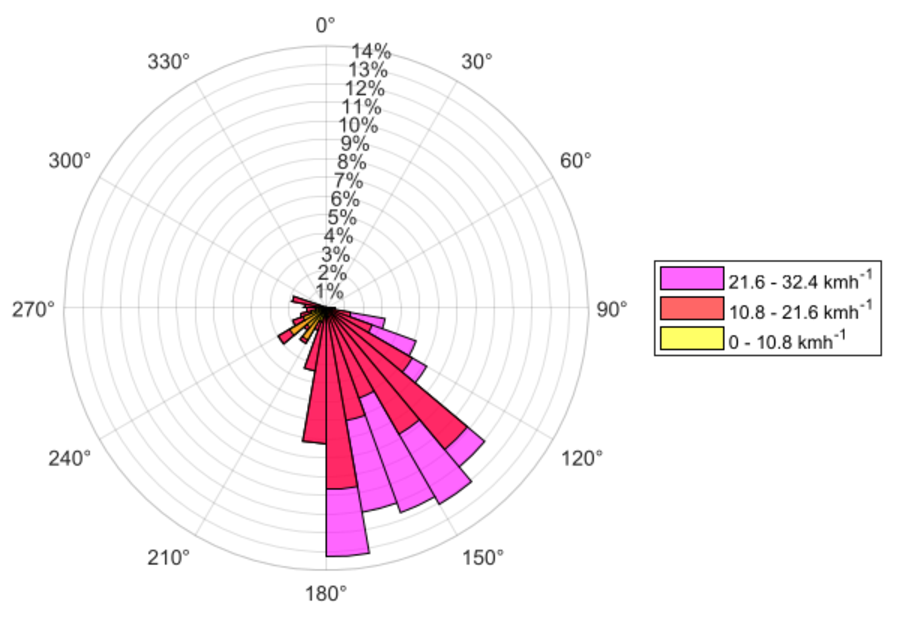
\includegraphics[width=0.8\textwidth]{img/Windrose.pdf}
%	\caption{Wind data expressed in a windrose diagram.}
%	\label{fig:Windrose}
%\end{figure}
%\begin{figure}[htbp]
%	\centering
%	\pgfplotsset{
	polar bar/.style={
		scatter,
		draw=none,
		mark=none,
		visualization depends on=rawy\as\rawy,
		area legend,
		legend image code/.code={%
			\fill[##1] (0cm,-0.1cm) rectangle (0.6cm,0.1cm);
		},
		/pgfplots/scatter/@post marker code/.add code={}{
			\pgfmathveclen{\pgf@x}{\pgf@y}
			\edef\radius{\pgfmathresult}
			\fill[]
			(\pgfkeysvalueof{/data point/x},-\pgfkeysvalueof{/data point/y})
			++({\pgfkeysvalueof{/data point/x}-#1/2},\pgfkeysvalueof{/data point/y})
			arc [start angle=\pgfkeysvalueof{/data point/x}-#1/2,
			delta angle=#1,
			radius={\radius pt}
			]
			-- +({\pgfkeysvalueof{/data point/x}+#1/2},-\rawy)
			arc [start angle=\pgfkeysvalueof{/data point/x}+#1/2,
			delta angle=-#1,
			radius={
				(\pgfkeysvalueof{/data point/y} - \rawy) / \pgfkeysvalueof{/data point/y} * \radius pt
			}
			]
			--cycle;
		}
	},
	polar bar/.default=30
}

\begin{tikzpicture}
	\begin{polaraxis}[
		xtick={0,45,...,315},
%		xticklabels={E,NE,N,NW,W,SW,S,SE},
		ytick=\empty,
%		legend entries={0 to 0.5, 0.5 to 2, 2 to 4, 4 to 6},
%		cycle list={cyan!20, cyan!50, cyan, cyan!50!black, cyan!20!black},
%		legend pos=outer north east
		]
%		\pgfplotsinvokeforeach{1,...,6}{
%			\addplot +[polar bar=17, stack plots=y]
%			table [x expr=-\thisrowno{0}+90, y index=#1] {frequencies.csv};
%		}
	\end{polaraxis}
\end{tikzpicture}
%	\caption{TODO.}
%	\label{fig:windrose}
%\end{figure}

%\clearpage
\newpage
\section{Official Rules}
\label{sec:bwscRules}
The BWSC has its own specific rules that can be downloaded on this link~\cite{bwscRules:2022webpage}. Not only they shape the opportunities and challenges that arise in this competition, but also ignoring or violating them can result in penalties or disqualification. Thus, it is of high importance to take them into consideration when making decisions and developing a plan.

The list of relevant rules can be divided into three categories based on their domain of application: time, space, and general. In the following paragraphs, only the rules that are relevant to the objectives of this thesis are listed.

\paragraph{Time domain}
The rules in the time domain pertain to the timing of various actions and events, such as when it is allowed to drive or permitted to tilt the car deck towards the sun:
\begin{itemize}
	\item The driving time on Day 1 is allowed between 10:00 and 17:00 (Rule 3.20.1).
	\item The driving time after Day 1 is allowed between 08:00 and 17:00 (Rule 3.20.2).
	\item From 15 minutes before sunrise until 15 minutes after sunset, teams are allowed to tilt the deck of their car towards the sun to recharge the batteries (Rule 3.27.8).
\end{itemize}
\paragraph{Space domain}
The rules in the space domain relate to the physical location of the car and its actions, such as the maximum speed limit on different types of roads or the requirement to stop at certain locations:
\begin{itemize}
	\item There are nine control stops at fix locations, where every team must stop for 30 minutes. In the case that a control stop is reached after 16:30, the time difference has to be recovered the next day starting from 08:00. For instance, if a team stops at 16:50, the next day it can start driving at 08:20 (Rule 3.26.1).
	\item Teams must not drive faster than the maximal allowed speed (Rule 3.31.7).
\end{itemize}
\paragraph{General}
The general rules are not specific to either time or space, but rather apply to the competition as a whole:
\begin{itemize}
	\item Teams can start their race with fully charged batteries (Rule 1.5.2).
	\item Teams should be able to sustain a minimal driving speed for open road of at least $v_\mathrm{min} = \unitfrac[60]{km}{h}$ (Rule 3.29.1).
\end{itemize}

